\section{Cross-Domain Replication: Radio Modulation Classification}
\label{sec:rf}

\subsection{Motivation}
The recall cliff could be a property of image classifiers, of convolutional
feature hierarchies, or of the particular detectors we use. To test whether it is
a property of deletion under partial poison, we repeat the core experiment in a
different modality: automatic modulation classification (AMC) on RadioML
2016.10a \cite{radioml,radioml_jstsp}. AMC is a natural second domain for this
question. Models are trained on large captures that may come from crowd-sourced
or third-party receivers, a poisoned capture is cheap to produce, and a backdoor
that maps a specific waveform to a fixed modulation label is a plausible
integrity attack on a receiver. Adversarial and poisoning threats to wireless
classifiers are an active concern in their own right \cite{sadeghi,flowers}, but
backdoor removal under imperfect detection has not, to our knowledge, been
characterised as a function of recall in this domain. The defence pipeline is the
same: detect, form a forget set, remove.

The protocol is summarised in Section~\ref{sec:protocol}. Eleven modulation
classes, SNR from $-20$ to $18$\,dB, $2\times128$ I/Q windows, unit-energy
normalisation, a three-block one-dimensional CNN, 5\% poison to BPSK, and a fixed
burst trigger that sets $I{=}0.9$ and $Q{=}{-}0.9$ on the last eight samples.
Three seeds vary poison placement and initialisation; the 80/20 split is fixed.
The same four methods and the same $(r,p)$ cells are used as in the image study,
including the precision-0.7 probe at $r{=}0.75$.

One feature of this domain changes how the results must be read. RadioML is
evaluated per SNR, and at low SNR the clean classifier is close to chance. We
report per-SNR numbers because they are the domain's native metric, but we mark
the near-chance region explicitly and restrict the interpretation of the recall
tolerance to SNR at or above $-6$\,dB. A defence that reports a low ASR on a
classifier that cannot classify is not a defence.

\subsection{The Attack and the Base Model}
The poisoned base model reaches ASR 99.54\% at 57.66\% clean accuracy, and its
per-SNR ASR is between 98.61\% and 100.00\% at every SNR from $-20$ to $18$\,dB.
That flatness is expected for a trigger that overwrites the end of the window:
the model can learn to read the burst regardless of the noise on the rest of the
signal. Clean accuracy, by contrast, depends strongly on SNR: 8.45\% at
$-20$\,dB, 10.5\% at $-16$, 23.4\% at $-10$, 48.2\% at $-6$, 63.2\% at $-4$,
82.2\% at $0$, and 85--87\% from 4\,dB upward. At $-20$\,dB the classifier is at
chance (9.1\% for eleven classes), so an ASR of 100\% is not evidence that the
backdoor is sophisticated; it is evidence that the trigger is easier to read than
the signal.

\subsection{Deletion Replicates the Cliff}
Table~\ref{tab:rf} and Fig.~\ref{fig:rf} report the removal results. Deletion
works when the forget set is complete: retraining on the retained set with every
poisoned sample removed reaches ASR $2.90\pm1.43\%$ at $r{=}1$ with clean
accuracy $56.83\pm0.57\%$. At $r{=}0.75$ its ASR is $97.16\pm1.84\%$; at $r{=}0.5$
it is $98.41\pm2.18\%$. The step is in the same place as in CIFAR-10: full recall
works, three-quarters recall does not. Fine-tune
never works, at any recall, with ASR $73.87$--$99.66\%$. On the SNR-averaged
cell, the two trigger-aware methods work down to $r{=}0.5$: the recipe reaches
$0.83\pm0.17\%$, $2.35\pm0.43\%$, and $4.02\pm0.86\%$ at the three recall levels,
and inoculation-only reaches $0.28\pm0.05\%$, $1.60\pm0.23\%$, and
$3.83\pm0.23\%$.
At the precision-0.7 cell ($r{=}0.75$), deletion is at 96.9--99.9\% ASR, the
recipe at 1.5--2.2\%, and inoculation-only at 1.4--1.8\%.

Two differences from the CIFAR results deserve comment. First, inoculation-only
succeeds in this domain, whereas on CIFAR-10 it left ASR at 17.67\%. The trigger
here is a simple additive burst on two channels, and the network's response to it
can be overwritten by presenting the burst with the correct label; the CIFAR patch
is spatial and interacts with many channels, and inoculation alone is not enough.
The cross-domain study therefore replicates the deletion cliff and the recipe's
tolerance, but it does not replicate the CIFAR ordering between the two
trigger-aware methods. We report the difference rather than pooling the domains.

Second, the radio task has a much lower clean-accuracy ceiling than CIFAR-10,
which compresses the utility side of the success criterion. A two-point budget
around a 56\% baseline is a tighter relative constraint than a two-point budget
around 89\%, but all methods here stay within about two points of the gold clean
accuracy, so the verdicts are driven by ASR. This is the regime in which the
recall cliff is easiest to see.

\begin{table}[t]
\centering
\caption{Cross-domain replication on RadioML AMC.}
\label{tab:rf}
\footnotesize
\setlength{\tabcolsep}{4.5pt}
\begin{tabular}{lcccc}
\toprule
\textbf{Method} & \textbf{$r{=}1.0$} & \textbf{$r{=}0.75$} & \textbf{$r{=}0.5$} & \textbf{Clean acc} \\
\midrule
Deletion & 2.90$\pm$1.43 & 97.16$\pm$1.84 & 98.41$\pm$2.18 & 56.75$\pm$0.79 \\
Fine-tune & 73.87$\pm$2.33 & 99.48$\pm$0.35 & 99.66$\pm$0.14 & 58.55$\pm$0.38 \\
Recipe & 0.83$\pm$0.17 & 2.35$\pm$0.43 & 4.02$\pm$0.86 & 57.36$\pm$0.50 \\
Inoc. only & 0.28$\pm$0.05 & 1.60$\pm$0.23 & 3.83$\pm$0.23 & 58.40$\pm$0.30 \\
\bottomrule
\end{tabular}
\par\vspace{1pt}\footnotesize\raggedright RadioML 2016.10a, 3 seeds, 5\% poison, synthetic I/Q trigger. Cells are ASR (\%) mean$\pm$s.d.\ over SNR and seeds; the last column is clean accuracy over all runs. The poisoned base reaches ASR 99.54\% at 57.66\% clean accuracy. The $r{=}1.0$ cell of the deletion row is the gold retrain. The recall cliff reproduces: deletion fails at $r\leq0.75$ (per-SNR ASR 90.3--100\% at $r{=}0.75$ and 89.6--100\% at $r{=}0.5$), while trigger-aware repair keeps the SNR-averaged ASR below 5\% to $r{=}0.5$.
\end{table}


\begin{figure*}[t]
\centering
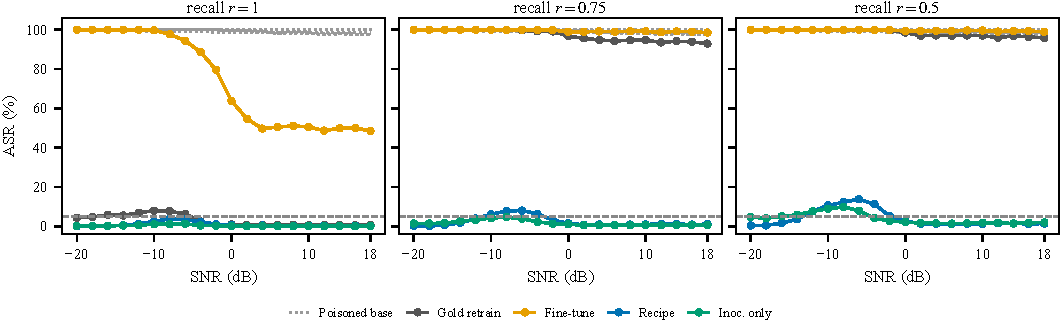
\includegraphics[width=\textwidth]{fig7_rf_asr.pdf}
\caption{ASR versus SNR on RadioML 2016.10a for recall 1.0, 0.75, and 0.5
(mean over three seeds). Deletion succeeds only at full recall (ASR $2.9\%$); at
partial recall its ASR is 90.3--100\%. Fine-tuning never removes the backdoor;
both trigger-aware methods stay at or below 5\% at high SNR, with the recipe
rising at mid SNR as Fig.~\ref{fig:rfheat} shows.}
\label{fig:rf}
\end{figure*}

\subsection{The Tolerance as a Function of SNR}
Fig.~\ref{fig:gamma} plots $\gstar$, the smallest recall at which a method
reaches ASR $\leq5\%$, as a function of SNR. Unlike $\rstar$, $\gstar$ carries no
utility budget: below $-10$\,dB the clean task is itself near chance, so a
two-point accuracy budget would not be meaningful. Clean accuracy is reported
separately in Table~\ref{tab:rf}. The oracle retrain has
$\gstar{=}1.0$ wherever it is defined, and it is undefined between $-16$ and
$-6$\,dB because the oracle model itself sits above 5\% ASR there
(5.45--7.87\%). That undefined region is not a failure of the retrain; it is a
statement that the attack is weak enough at those SNRs that the 5\% threshold
cannot separate a defended model from an undefended one. The two endpoints at
$-20$ and $-18$\,dB, where the oracle reports 4.26\% and 4.63\%, are also
degenerate: gold clean accuracy there is 8.4\% and 10.3\%, at or near chance. We mark
the whole region from $-20$ to $-10$\,dB as near-chance in the figure.

For the trigger-aware methods $\gstar$ is defined in every bin, and the profile
is U-shaped: the requirement is lowest at high SNR, rises through the mid range,
and is uninformative where the clean task is near chance. The recipe has
$\gstar{=}0.75$ at $-12$\,dB, $1.0$ at $-10$ to $-4$\,dB, $0.75$ at $-2$\,dB,
and $0.5$ from $0$\,dB upward. Inoculation-only has a similar profile, between
0.5 and 0.75. Fine-tuning has no $\gstar$: its best cell never falls below
48.5\%. The practical reading is narrower than a single recall number. Above
$0$\,dB, recall 0.5 suffices for trigger-aware repair; at $-12$ and $-2$\,dB the
requirement is 0.75, and between $-10$ and $-4$\,dB it is 1.0; below $-10$\,dB
the clean task is near chance and the criterion is vacuous. Deletion is
insufficient at every SNR at any recall below 1.0. A detector requirement stated
as one number is therefore itself an average over the operating SNR; the
deployment quantity is $\gstar$ as a function of SNR.

\begin{figure}[t]
\centering
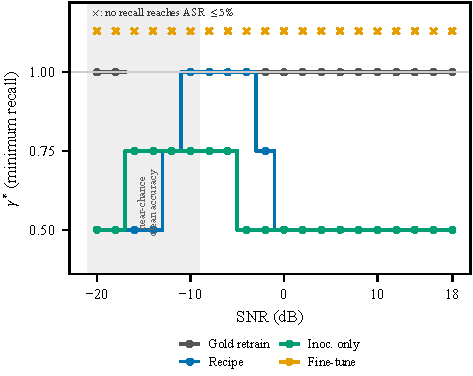
\includegraphics[width=\columnwidth]{fig8_rf_gamma.pdf}
\caption{$\gstar$ (minimum recall reaching ASR $\leq5\%$) versus SNR. Crosses
mark SNRs where no recall qualifies. The shaded region is near-chance clean
accuracy, where the 5\% criterion is vacuous.}
\label{fig:gamma}
\end{figure}

\subsection{Per-SNR Structure}
Fig.~\ref{fig:rfheat} shows every cell as a heatmap. Three structures are
visible. First, the fine-tune row is saturated at the partial-recall columns and
weakens only at $r{=}1$, where it falls from about 100\% in the near-chance bins
to 48.5\% at 18\,dB. That is the CIFAR-10 fine-tuning result at higher
resolution: even its best cell is ten times the 5\% threshold. Second, the
retrain row, which is the oracle at $r{=}1$ and partial deletion below it, turns
from blue to red between the first and second columns at every SNR: it is at
90.3--100\% at $r{=}0.75$ and 89.6--100\% at $r{=}0.5$. Third, the two
trigger-aware rows are blue across the band, but not uniformly. The lighter patch
between $-12$ and $-2$\,dB at $r{=}0.5$ is the mid-SNR hump: the recipe's per-SNR
ASR rises to 13.8\% at $-6$\,dB, even though the SNR-averaged cell mean is
4.02\%.

Fig.~\ref{fig:rfclean} explains why the left edge of the heatmap cannot be read
as a defence. In the shaded region below $-10$\,dB the three curves are
indistinguishable, and at $-20$ and $-16$\,dB they sit within 1.5 points of
chance. Above $-6$\,dB the recipe tracks gold within 4.3 points, so the mid-SNR
hump is a real removal failure on a task the network can perform, not a
side-effect of chance-level features.

\begin{figure*}[t]
\centering
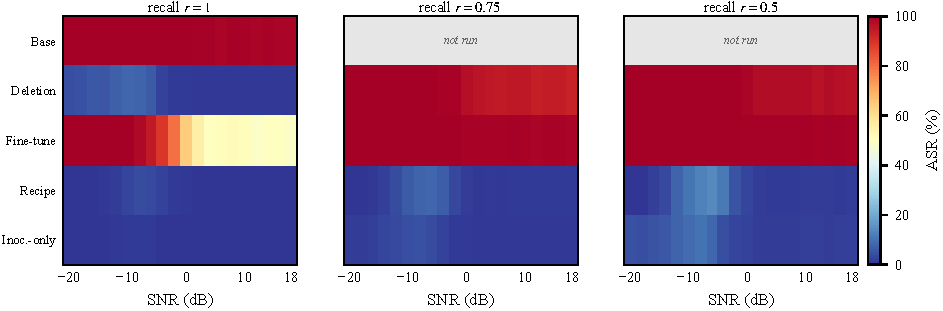
\includegraphics[width=\textwidth]{fig19_rf_heatmap.pdf}
\caption{ASR by SNR and recall for the radio study (mean over three seeds). The
retrain row is the oracle at $r{=}1$ and partial deletion at the lower recalls;
the base row was not run at partial recall (grey). Fine-tuning is saturated
except at full recall above 0\,dB; both trigger-aware methods are blue across the
band, with a lighter patch for the recipe at mid SNR.}
\label{fig:rfheat}
\end{figure*}

\begin{figure}[t]
\centering
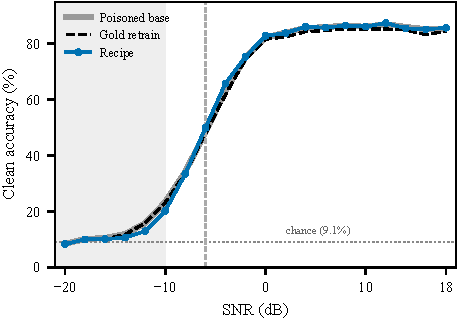
\includegraphics[width=\columnwidth]{fig20_rf_clean.pdf}
\caption{Clean accuracy versus SNR for the poisoned base, the gold retrain, and
the recipe at $r{=}1$. The three curves are nearly indistinguishable; the shaded
region below $-10$\,dB is near chance and the dashed vertical line marks
$-6$\,dB, the lower edge of the interpretable range.}
\label{fig:rfclean}
\end{figure}

\subsection{What the Radio Study Does and Does Not Show}
The study shows that the recall cliff is not specific to images, to
two-dimensional convolutions, or to the two CIFAR detectors. It appears in a
one-dimensional I/Q classifier with a different optimiser, a different poison
mechanism, and a per-SNR evaluation. It also shows that the recipe's tolerance is
not an artefact of the CIFAR architecture, although the simpler trigger makes
inoculation alone sufficient here.

It does not show that the result transfers to over-the-air signals. The trigger
is a digital burst applied before normalisation, not a hardware impairment; the
model is small; the dataset is a standard benchmark with a fixed split; and the
per-SNR bins contain different numbers of samples. These are ordinary
external-validity limits, and we list them rather than claim more than the
experiment supports. Within those limits, the radio study is the strongest
evidence in the paper that the cliff is a property of deletion under partial
poison rather than a property of one benchmark.
